
\documentclass[submit]{harvardml}

% Put in your full name and email address.
\name{Timothy Kang}
\email{tkang01@college.harvard.edu}

% List any people you worked with.
\collaborators{%
Jeff Chang
}

% You don't need to change these.
\course{CS181-S16}
\assignment{Assignment \#4}
\duedate{5:00pm Feb 1, 2016}

\usepackage[OT1]{fontenc}
\usepackage[colorlinks,citecolor=blue,urlcolor=blue]{hyperref}
\usepackage[pdftex]{graphicx}
\usepackage{subfig}
\usepackage{fullpage}
\usepackage{palatino}
\usepackage{mathpazo}
\usepackage{amsmath}
\usepackage{amssymb}
\usepackage{color}
\usepackage{todonotes}
\usepackage{listings}
\usepackage{common}
\usepackage{bm}

\usepackage[mmddyyyy,hhmmss]{datetime}

\definecolor{verbgray}{gray}{0.9}

\lstnewenvironment{csv}{%
  \lstset{backgroundcolor=\color{verbgray},
  frame=single,
  framerule=0pt,
  basicstyle=\ttfamily,
  columns=fullflexible}}{}

\begin{document}
\begin{center}
{\Large Homework 4: Clustering}\\
\end{center}

There is a mathematical component and a programming component to this homework.
Please submit ONLY your PDF to Canvas, and push all of your work to your Github
repository. If a question requires you to make any plots, please
include those in the writeup.


%%%%%%%%%%%%%%%%%%%%%%%%%%%%%%%%%%%%%%%%%%%%%
% Problem 1
%%%%%%%%%%%%%%%%%%%%%%%%%%%%%%%%%%%%%%%%%%%%%
\begin{problem}[The Curse of Dimensionality, 4pts]
In~$d$ dimensions, consider a hypersphere of unit radius, centered at zero,
which is inscribed in a hypercube, also centered at zero, with edges of length
two.  What fraction of the hypercube's volume is contained within the
hypersphere?  Write this as a function of~$d$.  What happens when~$d$ becomes
large?
\end{problem}

\subsection*{Solution}

We begin with the volume of an $n$-ball, which was taken from the relevant Wikipedia page:
	$$V_{n-\text{ball}} = \frac{\pi^{\frac{d}{2}}}{\Gamma\left(\frac{d}{2} + 1\right)}$$
The volume of the hypercube is trivial: $V_{\text{hypercube}} = 2^d$. From here, finding the fraction of the hypercube's volume that is contained within the hypersphere is simply a matter
of dividing the volume of the $n$-ball by the volume of the hypersphere:
	$$\text{fraction contained} = \frac{\pi^{\frac{d}{2}}}{\Gamma\left(\frac{d}{2} + 1\right)} \cdot
	\frac{1}{2^d}$$
Now we take the limit as $d \rightarrow \infty$:
	\begin{align*}
		\lim_{d \rightarrow \infty}  \frac{\pi^{\frac{d}{2}}}{\Gamma\left(\frac{d}{2} + 1\right)} \cdot
	\frac{1}{2^d} &= \lim_{d\rightarrow \infty}  \frac{\pi^{\frac{d}{2}}}{2^{\frac{d}{2}}} \cdot \frac{1}{2^{\frac{d}{2}}} \cdot \frac{1}{{\Gamma\left(\frac{d}{2} + 1\right)}}\\
	&= \lim_{d\rightarrow \infty} \frac{\left(\frac{\pi}{2}\right)^{\frac{d}{2}}}{2^{\frac{d}{2}}}
	 \cdot \frac{1}{{\Gamma\left(\frac{d}{2} + 1\right)}}\\
	 &\rightarrow 0
	\end{align*}
We know that the limit goes to 0 because $\frac{\pi}{2} \approx 1.57 < 2$, and the Gamma function is equivalent to a factorial. Therefore, the limit goes to 0. \\ \\
Intuitively, an $n$-ball with unit radius can be modeled as 
	$$x^2_1 + \dots + x^2_n = 1$$
As the number of dimensions increases, more and more of the $x$'s will need to be closer to 0. With a hypercube, the corners are still at $\pm 1$, regardless of how many dimensions, so the hypersphere captures less and less of the hypercube's volume as the dimensions increase. 	
%%%%%%%%%%%%%%%%%%%%%%%%%%%%%%%%%%%%%%%%%%%%%
\newpage
\begin{problem}[Norms, Distances, and Hierarchical Clustering, 5 pts]

  Consider the following four data points, belonging to three clusters: the
  black cluster $((x_1, y_1) = (0.1, 0.5) $ and $(x_2, y_2) = (0.35, 0.75))$,
  the red cluster $(x_3, y_3) = (0.28, 1.35)$ cluster, and the blue cluster
  $(x_4, y_4) = (0, 1.01)$.

  \begin{center} 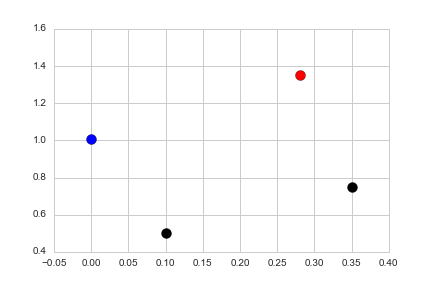
\includegraphics[scale=.4]{scatterplot.png} \end{center}
  At each step of hierarchical clustering, the two most similar (or least
  dissimilar) clusters are merged together. This step is repeated until there is
  one single group. Different distances can be used to measure group
  dissimilarity. Recall the definition of the $l_1$, $l_2$, and $l_{\infty}$
  norm:
  \begin{itemize}
    \item For $\mathbf{x} \in \mathbb{R}^n, \| \mathbf{x} \|_1 = \sum_{i = 1}^n
      |x_i|$
    \item For $\mathbf{x} \in \mathbb{R}^n, \| \mathbf{x} \|_2 = \sqrt{\sum_{i =
      1}^n x_i^2 }$
    \item For $\mathbf{x} \in \mathbb{R}^n, \| \mathbf{x} \|_{\infty} = \max_{i
      = 1}^n |x_i|$
  \end{itemize}
  Also recall the definition of single-link distance, complete-link distance,
  and average-link distance between two clusters:
  \begin{itemize}
    \item Single-link clustering: for clusters $G$ and $H$, $d_{S}(G, H) =
    \min_{i \in G, j\in H} d(i, j)$
    \item Complete-link clustering: for clusters $G$ and $H$, $d_{C}(G, H) =
    \max_{i \in G, j\in H} d(i, j)$
    \item Average-link clustering: for clusters $G$ and $H$, $d_{A}(G, H) =
      \frac{1}{|G| |H|} \sum_{i\in G}\sum_{j \in H} d(i, j)$
  \end{itemize}
  \paragraph{Warm up question.} \noindent Draw the 2D unit sphere for each norm,
  defined as $\mathcal{S} = \{x \in \mathbb{R}^2: \|x\| = 1 \}$. Feel free to do
  it by hand, take a picture and include it in your pdf.

  \paragraph{Main question.}
  \noindent For each norm ($l_1, l_2, l_\infty$) and each clustering method
  (single, complete, or average link clustering), specify which 2 clusters would
  be the first to merge.
\end{problem}
\subsection*{Solution}
\textbf{WARMUP QUESTION} \\ \\
\textbf{$\ell_1$ norm}: With this norm, the unit sphere is defined as
	$$|x_1| + |x_2| = 1$$
This yields four possible equations:
	\begin{align*}
		x_2 &= -x_1 - 1 \\
		x_2 &= x + 1 \\
		x_2 &= x_1 - 1\\
		x_2 &= 1-x_1
	\end{align*}
This produces the following unit sphere:\\
	\centerline{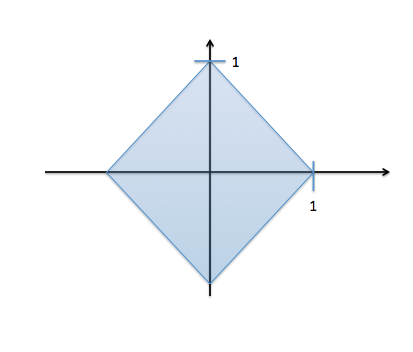
\includegraphics[scale=0.5]{./l1}}	
\textbf{$\ell_2$ norm}: With this norm, the unit sphere is defined as 
	$$\sqrt{x_1^2 + x_2^2} = 1 \implies x_1^2 + x_2^2 = 1$$
This is the familiar equation of a circle. \\ 
	\centerline{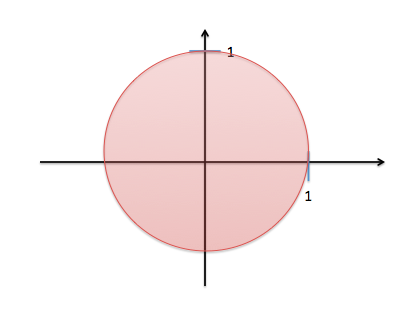
\includegraphics[scale=0.5]{./l2}}		
\textbf{$\ell_3$ norm}: With this norm, the unit sphere is defined as 
	$$\max (|x	_1|, |x_2|) =1$$
This means that we have $x_1 = \pm 1$ or $x_2 = \pm 1$. \\
	\centerline{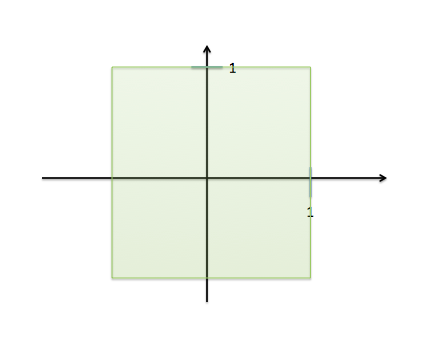
\includegraphics[scale=0.5]{./li}}
\textbf{MAIN QUESTION} \\ \\
Before we continue, we define the left point in the black cluster (0.1,0.5) as $A$  and the right point in the black cluster $(0.35,0.75)$ as $B$. Also, for single-link, we look for the minimum distance within each cluster comparison (i.e. within Black-Blue); for complete-link, we look for the maximum distance; and for average-link, we just average all of the distances with each cluster comparison. Then, we return the minimum distance between all three cluster comparisons. \\\\ 
\textbf{$\ell_1$ norm:} $\sum_i |x_i - y_i|$ (basically, add the differences between the $x$ and $y$ coordinates)\\ \\
	\underline{Inter-Cluster distances}
	\begin{itemize}
		\item \underline{Black-Blue}:
			\begin{itemize}
				\item \underline{A}: $|0.1 - 0|  + |0.5 - 1.01| = 0.61$
				\item \underline{B}: $|0.35- 0| + |0.75 - 1.01| = 0.61$
			\end{itemize}
		\item \underline{Black-Red}:
			\begin{itemize}
				\item \underline{A}: $|0.1 -0.28| + |0.5-1.35| = 1.03$
				\item \underline{B}: $|0.35-0.28| + |0.75-1.35| = 0.67$
			\end{itemize}
		\item \underline{Blue-Red}: $|0-0.28| + |1.01 - 1.35| = 0.62$
	\end{itemize}
	\underline{Clustering methods}
	\begin{itemize}
		\item \underline{Single link}:
			\begin{itemize}
				\item \underline{Black-Blue}: 0.61
				\item \underline{Black-Red}: 0.67
				\item \underline{Blue-Red}: 0.62
			\end{itemize}
		\textbf{Therefore, Black-Blue merge first}
		\item \underline{Complete link}:
			\begin{itemize}
				\item \underline{Black-Blue}: 0.61
				\item \underline{Black-Red}: 1.03
				\item \underline{Blue-Red}: 0.62
			\end{itemize}
		\textbf{Therefore, Black-Blue merge first}
		\item \underline{Average link}:
			\begin{itemize}
				\item \underline{Black-Blue}: 0.61
				\item \underline{Black-Red}: 0.85
				\item \underline{Blue-Red}: 0.62
			\end{itemize}
		\textbf{Therefore, Black-Blue merge first}	
	\end{itemize}
	
\noindent\textbf{$\ell_2$ norm:} $\sqrt{(x_1-x_2)^2 + (y_1-y_2)^2} $ (basically, the distance formula - all calculations were done using Wolfram alpha's distance formula calculator.)\\ \\
	\underline{Inter-Cluster distances}
	\begin{itemize}
		\item \underline{Black-Blue}:
			\begin{itemize}
				\item \underline{A}: 0.519
				\item \underline{B}: 0.436
			\end{itemize}
		\item \underline{Black-Red}:
			\begin{itemize}
				\item \underline{A}: 0.869
				\item  \underline{B}: 0.604
			\end{itemize}
		\item  \underline{Red-Blue}: 0.440
	\end{itemize}
	\underline{Clustering methods}
	\begin{itemize}
		\item \underline{Single link}:
			\begin{itemize}
				\item \underline{Black-Blue}: 0.436
				\item \underline{Black-Red}: 0.604
				\item \underline{Blue-Red}:  0.440
			\end{itemize}
		\textbf{Therefore, Black-blue merge first} 	
		\item  \underline{Complete link}:
			\begin{itemize}
				\item \underline{Black-Blue}: 0.519
				\item \underline{Black-Red}: 0.869
				\item \underline{Blue-Red}: 0.440
			\end{itemize}
		\textbf{Therefore, Blue-Red merge first}	
		\item  \underline{Average link}:
			\begin{itemize}
				\item \underline{Black-Blue}: 0.4775
				\item \underline{Black-Red}: 0.7365
				\item \underline{Blue-Red}: 0.440
			\end{itemize}		
		\textbf{Therefore, Blue-Red merge first}	
	\end{itemize}
\noindent\textbf{$\ell_{\infty}$ norm:}	This is the maximum of the absolute value of the difference between coordinates. 
	\underline{Inter-Cluster distances}
	\begin{itemize}
		\item \underline{Black-Blue}:
			\begin{itemize}
				\item \underline{A}: 0.51
				\item \underline{B}: 0.35
			\end{itemize} 
		\item \underline{Black-Red}:  
			\begin{itemize}
				\item \underline{A}: 0.85
				\item \underline{B}: 0.60
			\end{itemize}
		\item \underline{Red-Blue}: 0.34
	\end{itemize}
	\underline{Clustering methods}
	\begin{itemize}	
		\item \underline{Single link}:
			\begin{itemize}
				\item \underline{Black-Blue}: 0.35
				\item \underline{Black-Red}: 0.60
				\item \underline{Blue-Red}: 0.34
			\end{itemize}		
		\textbf{Therefore, Blue-Red merge first}	
		\item \underline{Complete link}:
			\begin{itemize}
				\item \underline{Black-Blue}: 0.51
				\item \underline{Black-Red}:  0.85
				\item \underline{Blue-Red}: 0.34
			\end{itemize}		
		\textbf{Therefore, Blue-Red merge first}	
		\item \underline{Average link}:
			\begin{itemize}
				\item \underline{Black-Blue}: 0.43
				\item \underline{Black-Red}: 0.725
				\item \underline{Blue-Red}: 0.34
			\end{itemize}			
		\textbf{Therefore, Blue-Red merge first}	
	\end{itemize}
\begin{table}[hbt]
\centering
\begin{tabular}{|l|l|l|l|}
\hline
         & $\ell_1$   & $\ell_2$   & $\ell_{\infty}$ \\ \hline
Single   & Black-Blue & Black-Blue & Red-Blue        \\ \hline
Complete & Black-Blue & Red-Blue   & Red-Blue        \\ \hline
Average  & Black-Blue & Red-Blue   & Red-Blue        \\ \hline
\end{tabular}
\end{table}
%%%%%%%%%%%%%%%%%%%%%%%%%%%%%%%%%%%%%%%%%%%%%

\newpage

\section*{K-Means [15 pts]}
Implement K-Means clustering from scratch.\footnote{That is, don't use a
third-party machine learning implementation like \texttt{scikit-learn};
\texttt{numpy} is fine.}. You have been provided with the MNIST dataset. You can
learn more about it at  \url{http://yann.lecun.com/exdb/mnist/}. The MNIST task
is widely used in supervised learning, and modern algorithms with neural
networks do very well on this task. We can also use MNIST for interesting
unsupervised tasks. You are given representations of 6000 MNIST images, each of
which are $28\times28$  handwritten digits. In this problem, you will implement
K-means clustering on MNIST, to show how this relatively simple algorithm can
cluster similar-looking images together quite well.

\begin{problem}[K-means, 15pts]
The given code loads the images into your environment as a 6000x28x28 array.
Implement K-means clustering on it for a few different values of $K$, and show
results from the fit. Show the mean images for each class, and by selecting a
few representative images for each class. You should explain how you selected
these representative images. To render an image, use the numpy imshow function,
which the distribution code gives an example of. Use squared norm as your
distance metric. You should feel free to explore other metrics along with
squared norm if you are interested in seeing the effects of using those. Also,
your code should use the entire provided 6000-image dataset (which, by the way,
is only 10\% of the full MNIST set).

Are the results wildly different for different restarts and/or different $K$?
Plot the K-means objective function as a function of iteration and verify that
it never increases.

Finally, implement K-means++ and see if gives you more satisfying
initializations (and final results) for K-means. Explain your findings.

As in past problem sets, please include your plots in this document. There may
be tons of plots for this problem, so feel free to take up multiple pages, as
long as it is organized.
\end{problem}
\subsection*{Solution}
\textbf{OBJECTIVE FUNCTION} 
	$$ J\left(\{\mathbf{r}_n\}^N_{n=1}, \{{\mu}_k\}^K_{k=1}\right) = \sum^N_{n=1} \sum^K_{k=1}
	r_{nk} \|\mathbf{x}_n - {\mu}_k\|^2_2$$
(The $\mu$ should be boldfaced)	
\begin{figure}[h]
	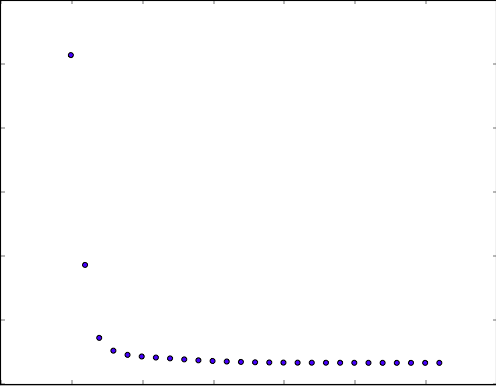
\includegraphics[scale=0.3]{./o/obj1} 
	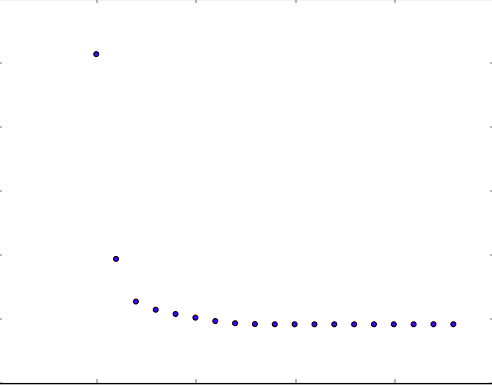
\includegraphics[scale=0.3]{./o/obj4} 
	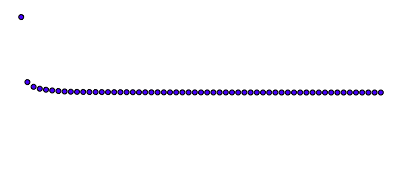
\includegraphics[scale=0.3]{./o/obj5} 
\end{figure}
\\\noindent From left-to-right: 
	\begin{itemize}
		\item $K = 10$ without KMeans++: 27 iterations and 76.39 seconds
		\item $K=5$ without KMeans++: 19 iterations and 25.30 seconds
		\item $K=10$ with KMeans++: 67 iterations and 109.02 seconds
	\end{itemize}
It is fairly obvious that the $K$-means objective function, as a function of iteration, is monotonically decreasing in the number of iterations (up to a certain point).\\ \\
\textbf{RESULTS OF K-MEANS WITHOUT K-MEANS++} \\
(Images are displayed from left-to-right)\\
\textbf{Set 1}: $K = 10$ - took 49 iterations and 139.18 seconds.  \\ 
\underline{Means:}
\begin{figure}[h]
	
\includegraphics[scale=0.1]{./m1/0}
	
\includegraphics[scale=0.1]{./m1/1}
	
\includegraphics[scale=0.1]{./m1/2}
	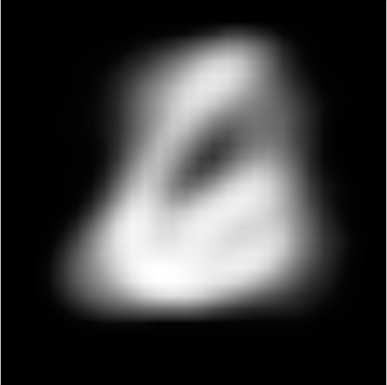
\includegraphics[scale=0.1]{./m1/3}
	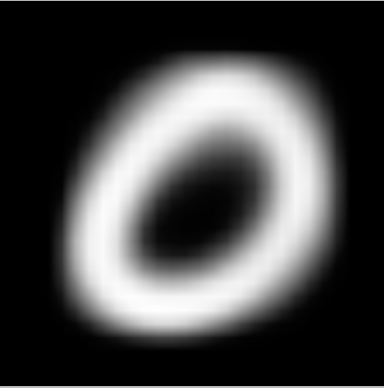
\includegraphics[scale=0.1]{./m1/4}
	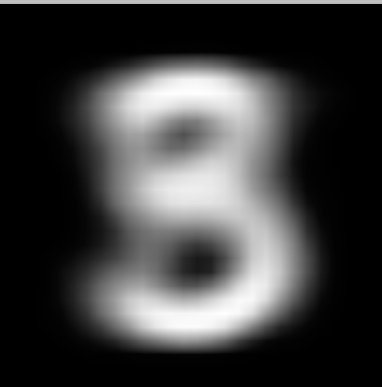
\includegraphics[scale=0.1]{./m1/5}
	
\includegraphics[scale=0.1]{./m1/6}
	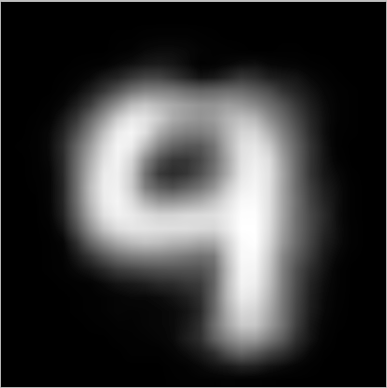
\includegraphics[scale=0.1]{./m1/7}
	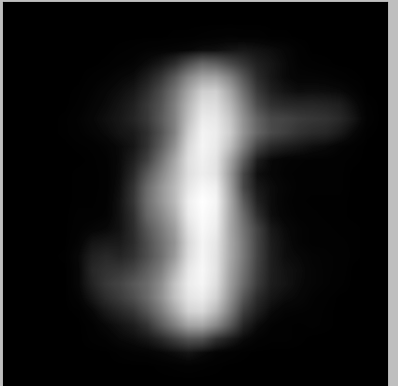
\includegraphics[scale=0.1]{./m1/8}
	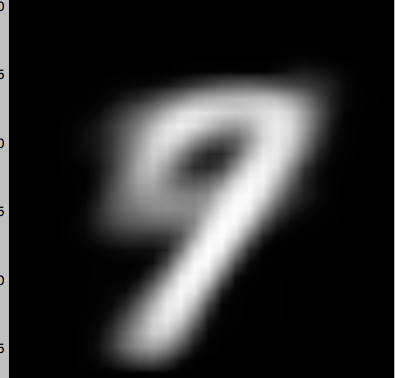
\includegraphics[scale=0.1]{./m1/9}
\end{figure}
\\ \noindent From left-to-right: 9. 5 or 3, 1, 6 or 2, 0, 3, 8, 9, 1, 7. \\ 
\underline{Representative Images:} \\ 
\centerline{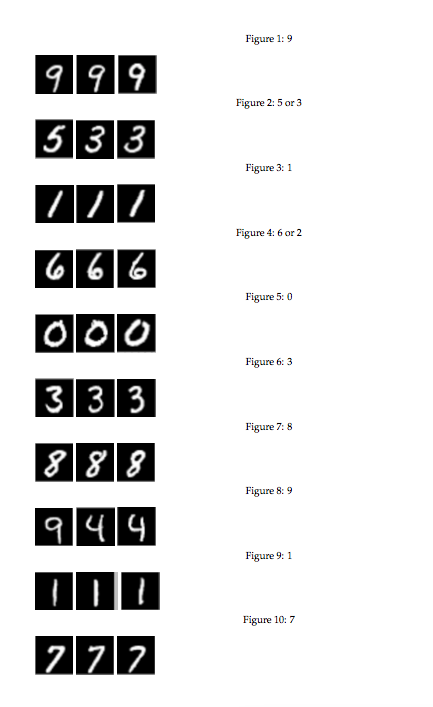
\includegraphics[scale=0.6]{./lmap}}
\textbf{Set 2:} $K = 10$ - took 42 iterations and 127.89 seconds. \\
\underline{Means:}\\ 
	\centerline{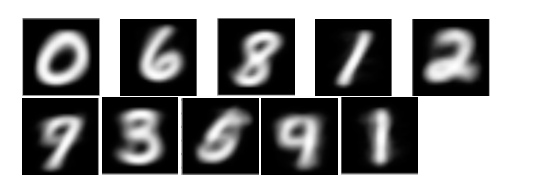
\includegraphics[scale=0.5]{./lmaa}}
\noindent From left-to-right: 0, 6, 8, 1, 2, 7 or 9, 3, 5, 9, 1.	\\
\underline{Representative Images:}\\
\centerline{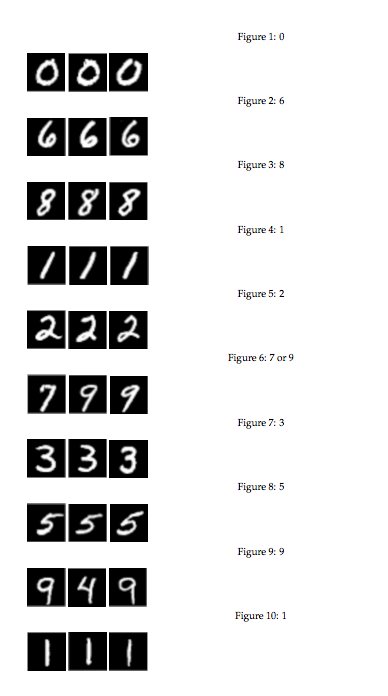
\includegraphics[scale=0.6]{./lmao}}

\noindent Between the two restarts (with same values of $K$), the results were largely the same. Both restarts took the same amount of time and produced, more-or-less, the same set of means. Also, the means were for the most part distinguishable: the images were not terribly blurry or merged (merged meaning overlapping numbers). It seems that K-means was not able to handle the numbers 4, 5, or 9 terribly well, as instances of these numbers tended to be merged with other numbers (that is, I would often get a 4 overlapped with 9). Similarly, 1 appeared quite frequently, largely because its structure is noticeable in other numbers (i.e. 7 or 5). Finally, the representative images for each cluster in both restarts seemed to largely match with the means that we returned.\\ 

\noindent\textbf{Set 3:} $K =3$ - took 52 iterations and 41.89 seconds. \\
\underline{Means:}\\
	\begin{figure}[h]
		
\includegraphics[scale=0.1]{./m3/0}
		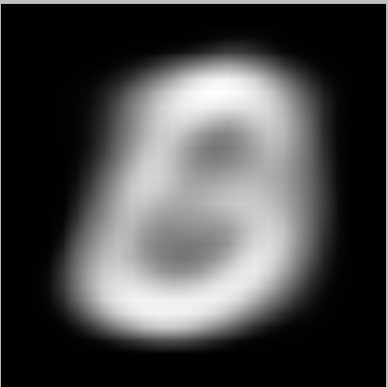
\includegraphics[scale=0.1]{./m3/1}
		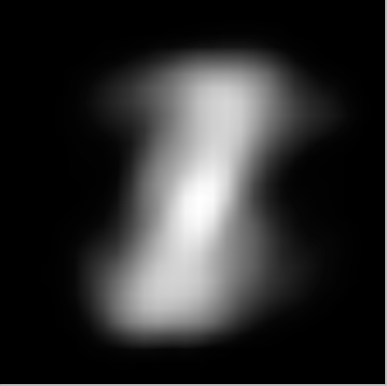
\includegraphics[scale=0.1]{./m3/2}
	\end{figure}
\\\noindent From left-to-right: 9; 8,3,6, ???; ???. \\
\underline{Representative Images:}\\
	\centerline{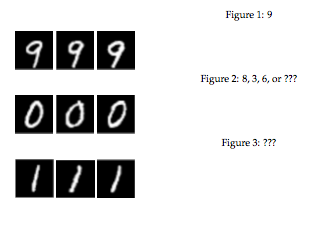
\includegraphics[scale=0.55]{./ayy}}
\noindent\textbf{Set 4:} $K=3$ - took 20 iterations and 17.37 seconds. \\
\underline{Means:}\\
	\begin{figure}[h]
		
\includegraphics[scale=0.1]{./m4/0}
		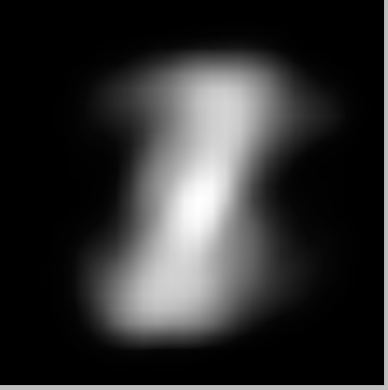
\includegraphics[scale=0.1]{./m4/1}
		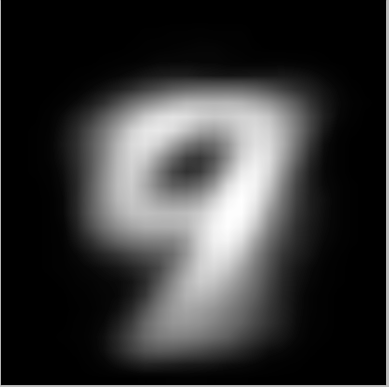
\includegraphics[scale=0.1]{./m4/2}
	\end{figure}
\\\noindent From left-to-right: ???, ???, 9 or 7.\\
\underline{Representative Images:}\\
	\centerline{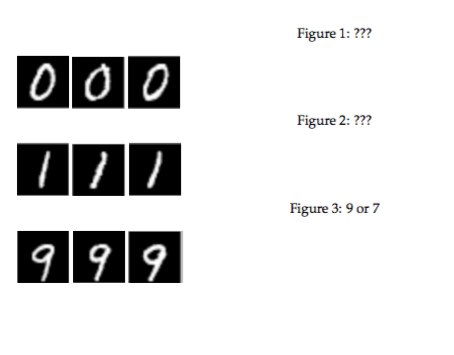
\includegraphics[scale=0.5]{./dafuq}}	
\noindent I ran the script 3 more times with $K = 3$ and got mostly the same results for the other 3 trials. All of the restarts produced identical means and representative images. Furthermore, for the means of the clusters, all of them seem to be overlapped images of numbers, which makes sense since only having three clusters means that some of the numbers will have to be grouped together.  \\ \\
\noindent\textbf{RESULTS OF K-MEANS WITH K-MEANS++} \\
 \textbf{Set 5:} $K=10$ - took 37 iterations and 89.24 seconds.\\
 \underline{Means:}\\
 	\begin{figure}[h]
		
\includegraphics[scale=0.1]{./m5/0}
		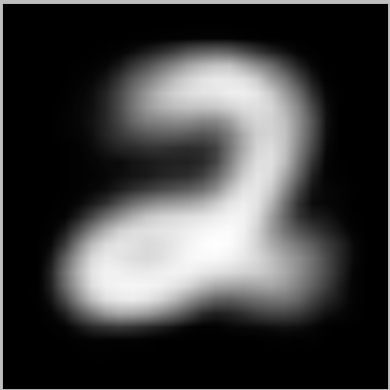
\includegraphics[scale=0.1]{./m5/1}
		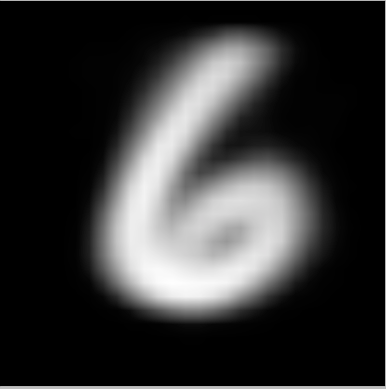
\includegraphics[scale=0.1]{./m5/2}
		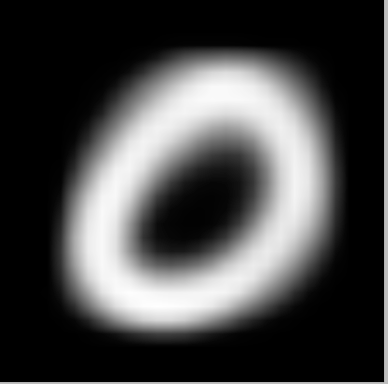
\includegraphics[scale=0.1]{./m5/3}
		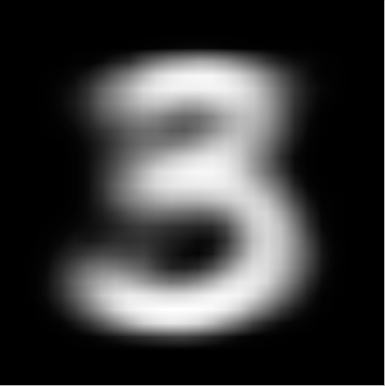
\includegraphics[scale=0.1]{./m5/4}
		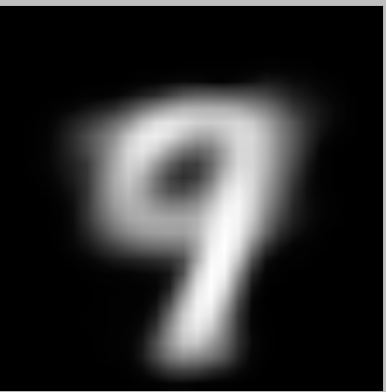
\includegraphics[scale=0.1]{./m5/5}
		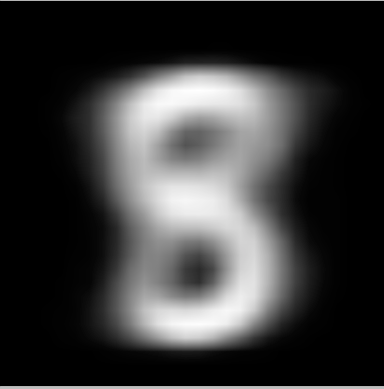
\includegraphics[scale=0.1]{./m5/6}
		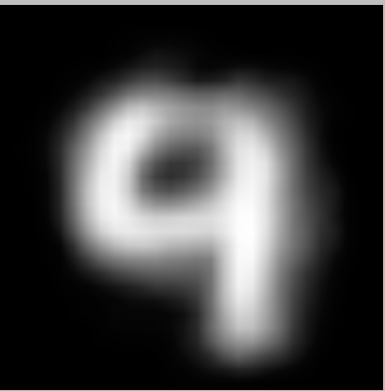
\includegraphics[scale=0.1]{./m5/7}
		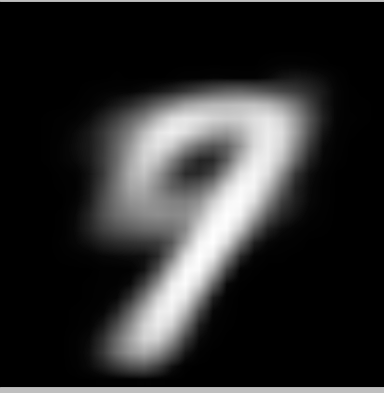
\includegraphics[scale=0.1]{./m5/8}
		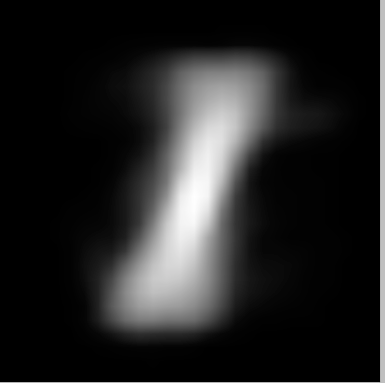
\includegraphics[scale=0.1]{./m5/9}
	\end{figure}
\\\noindent From left-to-right: 8,2,6,0,3,7,8,9,7,1. \\
\underline{Representative Images:}\\
	\centerline{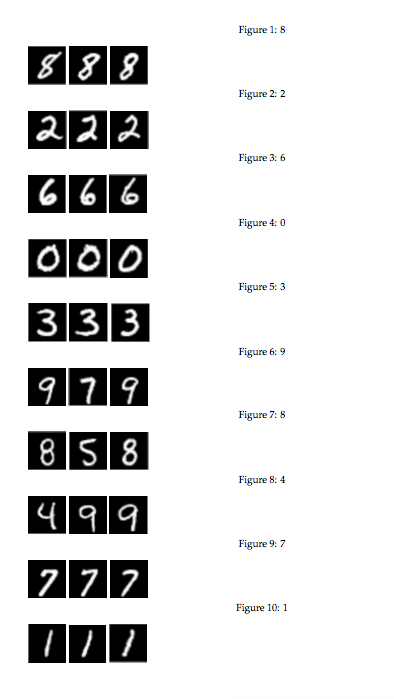
\includegraphics[scale=0.5]{./ALMOST}}
%\begin{figure*}[h]
%	\caption{8}
%	
\includegraphics[scale=0.1]{./r1/81}
%	
\includegraphics[scale=0.1]{./r1/82}
%	
\includegraphics[scale=0.1]{./r1/83}
%	\caption{2}
%	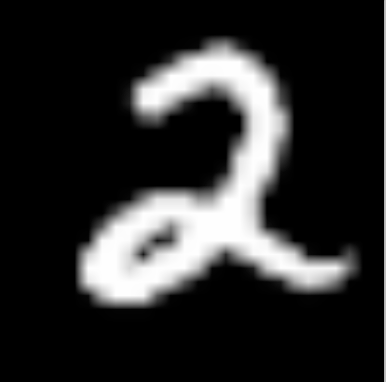
\includegraphics[scale=0.1]{./r1/21}
%	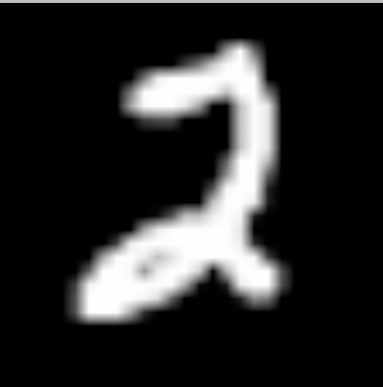
\includegraphics[scale=0.1]{./r1/22}
%	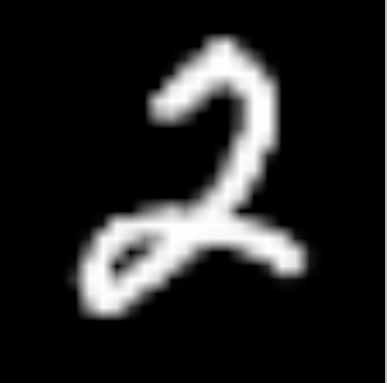
\includegraphics[scale=0.1]{./r1/23}
%	\caption{6}
%	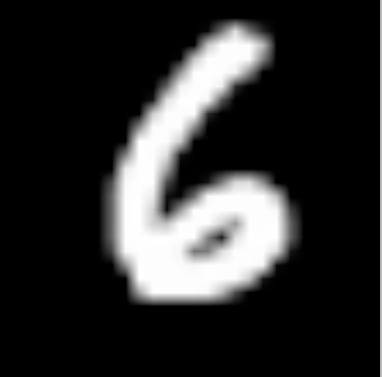
\includegraphics[scale=0.1]{./r1/61}
%	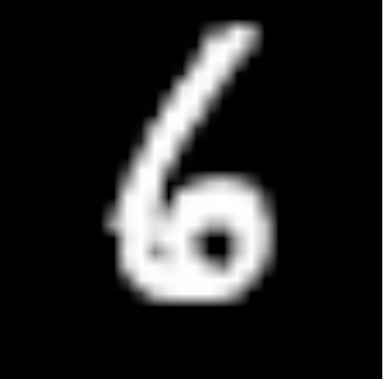
\includegraphics[scale=0.1]{./r1/62}
%	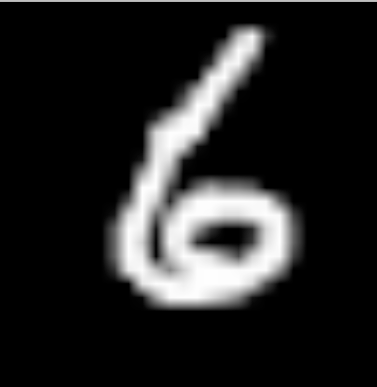
\includegraphics[scale=0.1]{./r1/63}
%	\caption{0}
%	
\includegraphics[scale=0.1]{./r1/01}
%	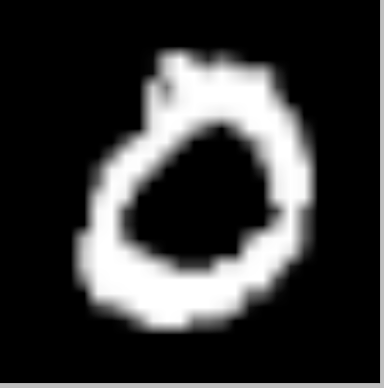
\includegraphics[scale=0.1]{./r1/02}
%	\includegraphics[scale=0.1]{./r1/03}
%	\caption{3}
%	\includegraphics[scale=0.1]{./r1/31}
%	\includegraphics[scale=0.1]{./r1/32}
%	\includegraphics[scale=0.1]{./r1/33}
%	\caption{9}
%	\includegraphics[scale=0.1]{./r1/91}
%	\includegraphics[scale=0.1]{./r1/92}
%	\includegraphics[scale=0.1]{./r1/93}
%	\caption{8}
%	\includegraphics[scale=0.1]{./r1/8a1}
%	\includegraphics[scale=0.1]{./r1/8a2}
%	\includegraphics[scale=0.1]{./r1/8a3}
%	\caption{4}
%	\includegraphics[scale=0.1]{./r1/41}
%	\includegraphics[scale=0.1]{./r1/42}
%	\includegraphics[scale=0.1]{./r1/43}
%	\caption{7}
%	\includegraphics[scale=0.1]{./r1/71}
%	\includegraphics[scale=0.1]{./r1/72}
%	\includegraphics[scale=0.1]{./r1/73}
%	\caption{1}
%	\includegraphics[scale=0.1]{./r1/11}
%	\includegraphics[scale=0.1]{./r1/12}
%	\includegraphics[scale=0.1]{./r1/13}
%\end{figure*} 

%Figure out how to load it into your environment and turn it into a set of
%vectors.  Run K-Means on it for a few different~$K$ and show some results from
%the fit.  What do the mean images look like?  What are some representative
%images from each of the clusters?  Are the results wildly different for
%different restarts and/or different~$K$?  Plot the K-Means objective function
%(distortion measure) as a function of iteration and verify that it never
%increases.
\noindent After reading the \texttt{Arthur and Vassilvitskii} paper (http://theory.stanford.edu/~sergei/papers/kMeansPP-soda.pdf), I realized that the primary benefit of $K$-means++ initialization is the improved runtime. Specifically, according to both the paper and Wikipedia page, ``With the k-means++ initialization, the algorithm is guaranteed to find a solution that is O(log k) competitive to the optimal k-means solution." While the initial selection process in $K$-means++ takes extra time, this allows the algorithm to converge to a quicker solution and reduce computation time. \\ \\
To confirm this, I ran $K$-means with 10 clusters and $K$-means++ initialization four more times and got the following results: 23 iterations and 47.466 seconds, 37 iterations and 62.034 seconds, 25 iterations and 72.041 seconds, and 26 iterations and 80.323 seconds. Overall, the $K$-means++ initialization did, in fact, improve runtime, and the results were just as accurate as $K$-means with random initialization. 
%\subsection*{4. Implement K-Means++ [4 pts]} mplement K-Means++ and see if it
%gives you more satisfying initializations for K-Means.  Explain your findings.
\newpage 

\begin{problem}[Calibration, 1pt]
Approximately how long did this homework take you to complete? \\ 
Finishing it took like 5 hours. Writing it up took another 3.
\end{problem}



\end{document}
